%---------------------------------------------------------------------
%Babitha Bokka
%---------------------------------------------------------------------
\documentclass[12pt]{article}
\usepackage{graphicx}
\usepackage{listings}
\usepackage{hyperref}
\usepackage{caption}
\graphicspath{ {images/} }

%Start Margins
\addtolength{\oddsidemargin}{-.875in}
\addtolength{\evensidemargin}{-.875in}
\addtolength{\textwidth}{1.75in}

\addtolength{\topmargin}{-.885in}
\addtolength{\textheight}{1.95in}
%End Margins

\begin{document}

%---------------------------------------------------------------------
%Making the title page
%---------------------------------------------------------------------
\begin{titlepage}

\title{INTRODUCTION TO WEBSCIENCES:\\*Assignment-1}
\author{Babitha Bokka}
\date{11 September 2014}
\maketitle

\end{titlepage}

%---------------------------------------------------------------------
%Table of contents
%---------------------------------------------------------------------
\tableofcontents
\newpage
%------------------------------------------------------------------
%Question 1
%------------------------------------------------------------------
\section{Question 1}
%\subsection{Description}
Demonstrate how to POST data to a webpage by using "curl" ,the server should take the arguments posted and generate a response. Take the response:
\begin{enumerate}
	\item Save it into a file
	\item Open the file in a browser and take a screen shot.
\end{enumerate}
%------------------------------------------------------------------
\subsection{Approach Towards the Solution}
"curl" is a command line tool to communicate with web servers.

\subsubsection{Test 1}
To demonstrate how "curl" can communicate with the webserver I have created a webpage which has to fields first and last name when you post the arguments by using the below command the serevr would take your commands and generate a  response I saved the response in a file.

\subsubsection{Test 2 }
The other way i tested the curl command is by posting the arguments(MIDAS ID:--- ;Password:---) and got the response from the server.And if you observe the gresponse.htm there is and error message which explains server sends 200 OK but doesn't like to communicate with the curl command.
%------------------------------------------------------------------
\subsection{Source Code}
\subsubsection{webTest.php}
\lstinputlisting[breaklines=True]{webTest.php}
\subsubsection{sucessPage.php}
\lstinputlisting[breaklines=True]{sucessPage.php}
%-------------------------------------------------------------------
\subsection{Solution}
\subsubsection{POST method}
Test 1:
\begin{verbatim}
curl -i -A "Mozilla/4.0" --data-urlencode "fname=babitha&lname=bokka&submit=ok" 
http://www.cs.odu.edu/~bbokka/curlTest/sucessPage.php/ > response.htm

Test 2:
curl -i -A "Mozilla/4.0" --data-urlencode "j_username=bbokk001&j_password=***&submit=Login" https://shibboleth.odu.edu/idp/Authn/MidasPreviousSession > save.htm
\end{verbatim}
\subsubsection{GET method}
\begin{verbatim}
curl -A "Mozilla/4.0" "http://www.cs.odu.edu/~bbokka/curlTest/sucessPage.php?fname=babitha & lname=bokka & submit=ok"

\end{verbatim} 
%-------------------------------------------------------------------
\newpage
\subsection{Output}
\subsubsection{response.htm}
\lstinputlisting[breaklines=True]{response.htm}
\subsubsection{gresponse.htm}
\lstinputlisting[breaklines=True]{gresponse.htm}
\subsection{Screen Shots}
\begin{figure}[ht]
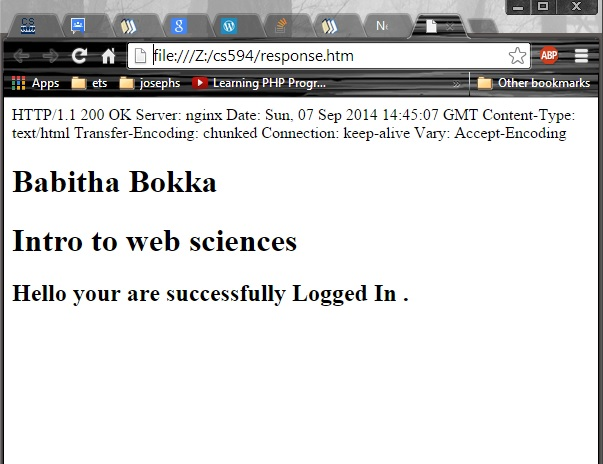
\includegraphics[scale=0.7]{responseScreenShot}
\centering
\caption{Test 1 Screen shot}
\end{figure}

\begin{figure}
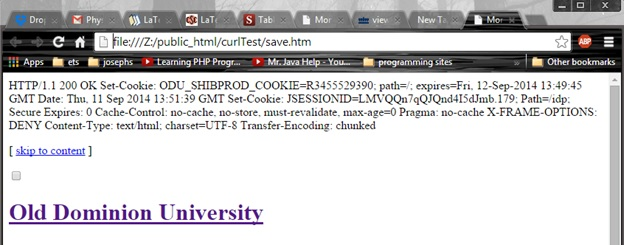
\includegraphics[scale=0.6]{gresponseScreenShot}
\centering
\caption{Test 2 Screen shot}
\end{figure}
\newpage
%------------------------------------------------------------------
%Question 2
%------------------------------------------------------------------
\section{Question 2}
%------------------------------------------------------------------
\subsection{Description}
Write a python program which takes the three arguments like\\* 
1.Team name\\*
2.Time to Sleep\\*
3.URI\\*
and get the scores of the respective team and the opposite team waits for the time and gets the scores untill you hit ctrl+c.
%------------------------------------------------------------------
\subsection{Approach Towards the Solution}
The aim of the program is to scrape sports webpages and get the sores of the given team.In order to scrape the webpages we have a beautiful library called Beautiful Soup which has many functions in it(contents , findChildren ,findAll etc...).The below python program uses Requests and beautiful Soup Library to get the contents of the webpage and extract the required data from the html.And to keep on updating the scores we halt the program by using time.sleep() function for the specified time.
 The below program get scores from the respective URI's\\*
\url{http://sports.yahoo.com/college-football/scoreboard/?week=2&conf=all}
\\*
\url {http://sports.yahoo.com/college-football/scoreboard/?week=1&conf=72}

\subsection{Python Code}
\subsubsection{A1.py}
\lstinputlisting[breaklines=True]{A1.py}

%------------------------------------------------------------------
\newpage
\subsection{Output}

\begin{figure}[ht]
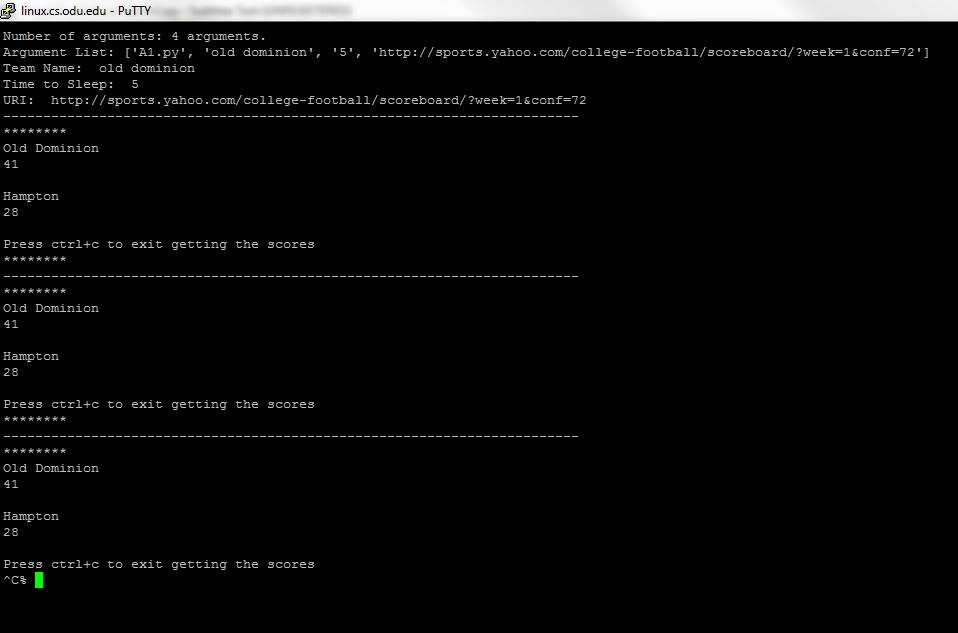
\includegraphics[scale=0.7]{programOutput}
\centering
\caption{Python Program Output}
\end{figure}
\newpage
%------------------------------------------------------------------
\section{Question 3}
%-------------------------------------------------------------------
\subsection{Problem Description:}
Given a graph determine the values of \\*
IN\\*
SCC\\*
OUT\\*
Tendrils\\*
Tubes\\*
Disconnected\\*
%-------------------------------------------------------------------
\subsection{Graph:}
\subsubsection{Diagram}
\begin{figure}[ht]
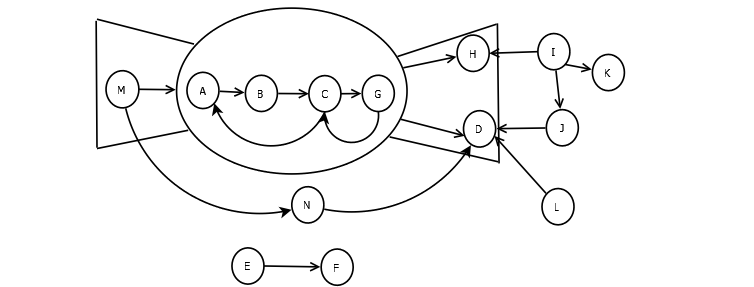
\includegraphics[scale=0.6]{graph}
\caption{Given graph in bow tie structure of web}
\centering
\end{figure}



%-------------------------------------------------------------------
\subsection{Values of :}
IN:1\\*
SCC:4\\*
OUT:2\\*
Tendrils:4\\*
Tubes:1\\*
Disconnected:2\\*
\newpage
%-------------------------------------------------------------------
\subsection{Definition}
From the broders paper and definition below :\\*
Definition:\\*
SCC: We say that a strongly connected component (SCC) in a directed graph is a
subset of the nodes such that: (i) every node in the subset has a path to every
other; and (ii) the subset is not part of some larger set with the property that
every node can reach every other
\\*\\*
IN: Nodes that can reach the giant SCC but cannot be reached from it — i.e., nodes
that are “upstream” of it.
\\*\\*
OUT: Nodes that can be reached from the giant SCC but cannot reach it — i.e., nodes
are “downstream” of it.
\\*\\*
Tendrils: The “tendrils” of the bow-tie consist of (a) the nodes reachable from IN that
cannot reach the giant SCC, and (b) the nodes that can reach OUT but cannot be
reached from the giant SCC. For example, the page My song lyrics in Figure 13.6 is
an example of a tendril page, since it’s reachable from IN but has no path to the giant
SCC. It’s possible for a tendril node to satisfy both (a) and (b), in which case it’s
part of a “TUBE” that travels from IN to OUT without touching the giant SCC. (For
example, if the page My song lyrics happened to link to Blog post about Company Z in
Figure 13.6, it would be part of a tube.)
\\*\\*
Disconnected: Finally, there are nodes that would not have a path to the giant SCC
even if we completely ignored the directions of the edges. These belong to none of the
preceding categories.
\\*\\*
\subsection{How are the nodes forming SCC, IN....?}
From the above definition SCC , has the strongly connected nodes if we apply this definition to the graph given that A , B, C, G are the strongly connected components where each and every node can be reached by every other node , the node M is the IN since that is only node which can reach the SCC and node H,D falls under OUT beacsue they are the only nodes that can be reached by SCC . The node N connects both IN and OUT so it forms the TUBE .Nodes E and F are not connected to SCC in any way so they are DISCONNECTED. Nodes I ,J,K,L are the OUT tendrils.
\newpage
%-------------------------------------------------------------------
%References
%-------------------------------------------------------------------
\bibliographystyle{plain}
\bibliography{A1_report}
\cite{*}


\end{document}